\documentclass[landscape]{slides}
%\AtBeginDocument{%
%  \pdfpageheight = \paperheight
%  \pdfpagewidth = \paperwidth
%}

\usepackage{txfonts}
\usepackage{color}
\usepackage{latexsym}
\usepackage{strikeout}
\ifx\pdfoutput\undefined
  \usepackage{graphicx}
\else
  \usepackage[pdftex]{graphicx}
  \DeclareGraphicsRule{*}{mps}{*}{}
\fi
%\usepackage{cgloss4e,gb4e}
%\usepackage[final]{pdfpages}

\usepackage{amssymb}

\font\manual=manfnt
\def\dbend{{\manual\char127}}   % dangerous bend sign

\raggedright

\definecolor{bgblue}{rgb}{0.04,0.39,0.53}

\newcommand{\argmax}[1]{\begin{array}{c}\mbox{arg max}\\#1\end{array}}

\begin{document}

\begin{slide}
\vspace{2in}
\begin{center}
\Large {\color{blue} Formal Language, Natural Language\\ and Tree Adjoining Grammars}\\
\vspace{2in}
\normalsize \color{red}Anoop Sarkar\\
{\tt anoop@cs.sfu.ca}
\end{center}
\end{slide}

\begin{slide}{\underline{Overview}}
\begin{itemize}
\item Tree Adjoining Grammars \[ \textrm{TAGs} \left\{ 
\begin{array}{l}
\textrm{Weak vs. Strong Generative Capacity}\\
\textrm{Natural Language and Complexity}\\
\textrm{Lexicalization of Grammars}
\end{array}
\right. \]
\item TAGs for Natural Languages
%%\item TAGs for Biological Sequences
\end{itemize}
\end{slide}

%\begin{slide}{The Chomsky Hierarchy}
%\begin{itemize}
%\item {\bf unrestricted} or {\bf type-0} grammars, generate the {\em
%recursively enumerable} languages, automata equals {\em Turing
%machines}
%\item {\bf context-sensitive} grammars, generate the {\em
%context-sensitive} languages, automata equals {\em Linear Bounded
%Automata}
%\item {\bf context-free} grammars, generate the {\em context-free}
%languages, automata equals {\em Pushdown Automata}
%\item {\bf regular} grammars, generate the {\em regular} languages,
%automata equals {\em Finite-State Automata}
%\end{itemize}
%\end{slide}

\begin{slide}{Strong vs. Weak Generative Capacity}
\begin{itemize}
\item {\bf Weak generative capacity} of a grammar is the set of
strings or the language, e.g. $0^n 1^n$ for $n \geq 0$
\item {\bf Strong generative capacity} is the set of structures
(usually the set of trees) provided by the grammar
\end{itemize}
\end{slide}

\begin{slide}{Strong vs. Weak Generative Capacity}
\begin{eqnarray}
S & \rightarrow & NP\ VP \\
VP & \rightarrow & V\ NP \mid VP\ ADV \\
NP & \rightarrow & David \mid peanuts \\
V & \rightarrow & likes \\
ADV & \rightarrow & passionately
\end{eqnarray}
\[ L(G) = \{ \textrm{David likes peanuts}, \textrm{David likes peanuts passionately} \} \]
\end{slide}

\begin{slide}{Derived Tree/Parse Tree}
\begin{center}
\includegraphics[width=6in]{figures.27}
\end{center}
\end{slide}

\begin{slide}{Derivation Tree}
\begin{center}
\includegraphics[width=8in]{figures.28}
\end{center}
\end{slide}

\begin{slide}{\underline{Tree Sets}: Given CFG, $G$, let $T(G)$ be the set of derived trees}
\begin{eqnarray}
S & \rightarrow & A\ B \nonumber \\
A & \rightarrow & a\ A \mid a \nonumber \\
B & \rightarrow & B\ b \mid b\nonumber 
\end{eqnarray}
\begin{center}
\includegraphics[height=3in]{figures.29}
\end{center}
Tree set $T$ shown here, $T=T(G)$
\end{slide}

\begin{slide}{\underline{Tree Sets}: Consider $T'$ below. There is no CFG $G$ such that $T(G)
  = T'$: {\color{red} Why?}}
\begin{center}
\includegraphics[height=4in]{figures.30}
\end{center}
\end{slide}

\begin{slide}{Local Tree Predicates}
\begin{eqnarray}
A & \rightarrow & \includegraphics[height=1in]{figures.31}\ \  \textrm{ if there is a
  right tree context A } \nonumber \\
A & \rightarrow & \includegraphics[height=1in]{figures.32}\ \  \textrm{ if there is a
  left tree context A } \nonumber \\
S & \rightarrow & \includegraphics[height=1in]{figures.34}\ \  \textrm{ no context needed } \nonumber 
\end{eqnarray}

Apply the predicates to trees and we can accept or reject trees. That is, we can {\em recognize} a tree set. Just like a grammar {\em recognizes} a set of strings, these predicates can recognize a set of trees.

\end{slide}

\begin{slide}{\dbend\ \underline{Tree Sets}}
\begin{center}
\includegraphics[height=4in]{figures.30}\\
However, $T'$ can be recognized by a finite-state bottom-up tree automaton
\end{center}
\end{slide}

\begin{slide}{\dbend\ Tree Sets of CFGs and Recognizable Sets}
\begin{itemize}
\item Recognizable Sets: Tree sets recognized by finite-state
  bottom-up tree automata: analogs of regular sets
\item Strings sets of recognizable sets are context-free languages
\item Recognizable sets are the same as tree sets of CFGs closed under
 relabelling homomorphisms (Thatcher, 1967)
\item Additional strong generative power of recognizable sets by
  introducing local tree predicates
\end{itemize}
\end{slide}

%\begin{slide}{Local Tree Predicates}
%\begin{center}
%\includegraphics[height=4in]{figures.30}
%\end{center}
%\end{slide}

\begin{slide}{Tree Sets of CFGs and Recognizable Sets}
\begin{itemize}
\item Surprisingly, even context-sensitive grammars when interpreted
  as local tree predicates can only {\em generate} the recognizable
  sets
\item Local sets = Tree sets for CFGs; Recognizable sets = Local sets plus relabeling of the nodes
\item Hence, CSGs when interpreted as ``filters'' on trees can only
  produce context-free languages (Peters and Ritchie, 1969; McCawley,
  1967)
\item Result can be strengthened to boolean combinations of CSG local tree
  predicates (Joshi, Levy and Yueh, 1972; Rogers, 1997)
\end{itemize}
\end{slide}

\begin{slide}{\underline{Overview}}
\begin{itemize}
\item Tree Adjoining Grammars \[ \textrm{TAGs} \left\{ 
\begin{array}{l}
\textrm{\strike{Weak vs. Strong Generative Capacity}}\\
\textrm{Natural Language and Complexity}\\
\textrm{Lexicalization of Grammars}
\end{array}
\right. \]
\item TAGs for Natural Languages
%%\item TAGs for Biological Sequences
\end{itemize}
\end{slide}

\begin{slide}{Natural Language and Complexity}
\begin{itemize}
\item We ask the question: {\em Does a particular formal language describe some aspect of human language}
\item Then we find out if that language {\bf isn't} in a particular
language class
\item For example, if we abstract some aspect of human language to the
formal language: $\{ w w^R \mid \textrm{ where } w \in \{a,b\}^\ast,
w^R \textrm{ is the reverse of } w \}$ we can then ask if it is
possible to write a regular expression for this language
\item If we can, then we can say that this particular example from
human language does not go beyond regular languages. If not, then we
have to go higher in the hierarchy (say, up to context-free languages)
\end{itemize}
\end{slide}

\begin{slide}{Strong vs. Weak Generative Capacity}
\begin{itemize}
\item If we consider strong generative capacity then the answer is
  somewhat easier to obtain 
\item For example, do we need nested dependencies to compute the
  semantics in a natural way?
\end{itemize}
\end{slide}

\begin{slide}{\dbend\ Strong vs. Weak Generative Capacity}
\begin{itemize}
\item However, strong generative capacity requires a particular
grammar and a particular linguistics theory of semantics or how
meaning is assigned (in steps or compositionally)
\item So, the stronger claim will be that some aspect of human
language when you consider {\em weak} generative capacity is not
regular
\item This is quite tricky: consider $L_1 = \{ a^n b^n \}$ is
context-free but $L_2 = \{ a^\ast b^\ast \}$ is regular and $L_1
\subset L_2$: so you could cheat and pick some subset of the language
which won't prove anything
\item Furthermore, the language should be {\em infinite}
\end{itemize}
\end{slide}

\begin{slide}{Strong vs. Weak Generative Capacity}
\begin{itemize}
\item Also, if we consider the {\em size} of a grammar then also the
answer is easier to obtain ($\ast$joyable, $\ast$richment). The CFG is
more {\em elegant} and smaller than the equivalent regular grammar:
\begin{eqnarray}
V &\rightarrow& X \nonumber \\
A &\rightarrow& X\ \textit{-able}~\mid~X\ \textit{-ment}\nonumber \\
X &\rightarrow& \textit{en-}\ NA \nonumber \\
NA &\rightarrow& \textit{joy}~\mid~\textit{rich} \nonumber
\end{eqnarray}
\item This is an engineering argument. However, it is related to the
problem of describing the human learning process. Certain aspects of
language are learned all at once not individually for each case.\\
{e.g., learning {\em enjoyment} automatically if {\em enrichment} was
learnt}
\end{itemize}
\end{slide}

\begin{slide}{Is Human Language a Regular Language}
\begin{itemize}
\item Consider the following set of English sentences (strings)
\begin{itemize}
\item $S = $ If $S_1$ then $S_2$
\item $S = $ Either $S_3$, or $S_4$
\item $S = $ The man who said $S_5$ is arriving today
\end{itemize}
\item Map {\em If, then} $\rightarrow a$ and {\em either, or}
$\rightarrow b$. This results in strings like $abba$ or $abaaba$ or
$abbaabba$
\item $L = \{ w w^R \mid \textrm{ where } w \in \{a,b\}^\ast, w^R
\textrm{ is the reverse of } w \}$
\end{itemize}
\end{slide}

%\begin{slide}{Human Language is not a Regular Language}
%\begin{itemize}
%\item Is $L = w w^R$ a regular language? To show something is {\em
%not} a regular language, we use the {\bf pumping lemma}: for any
%infinite set of strings generated by a FSA if you consider a long
%enough string from this set, there has to be a loop which visits the
%same state at least twice
%\item Thus, in a regular language $L$, there are strings $x, y, z$
%such that $x y^n z$ for $n \geq 0$ where $y \not= \epsilon$
%\item Let $L'$ be the intersection of $L$ with $aa^\ast bb
%aa^\ast$. Recall that RLs are closed under intersection, so $L'$ must
%also be a RL. $L' = a^n bb a^n$ \\ For any choice of $y$ (consider
%$a^i$ or $b^i$ or $a^i b$ or $b a^i$) the pumping lemma leads to the
%conclusion that $L'$ is {\bf not} regular.
%\end{itemize}
%\end{slide}

\begin{slide}{Human Language is not a Regular Language}
\begin{itemize}
\item Another example, also from English, is the set of center embedded structures\\
Think of $S \rightarrow a\ S\ b$ and the nested dependencies $a_1 a_2 a_3 b_3 b_2 b_1$
\item Center embedding in English:\\
{\em the shares that the broker recommended were bought} $\Rightarrow N_1 N_2 V_2 V_1$\\
{\em the moment when the shares that the broker recommended were bought has passed} $\Rightarrow N_1 N_2 N_3 V_3 V_2 V_1$
\item Can you come up with an example that has four verbs and corresponding number of nouns?
\end{itemize}
\end{slide}

\begin{slide}{Human Competence vs. Human Performance}
\begin{itemize}
\item What if no more than 3 or 4 center embedding structures are possible? Then the language is finite, so the language is no longer strictly context-free
\item The common assumption made is that human competence is represented by the context-free grammar, but human performance suffers from memory limitations which can be simulated by a simpler mechanism
\item The arguments about elegance, size and the learning process in humans also apply in this case
\end{itemize}
\end{slide}

\begin{slide}{Human Language is not a Context-Free Language}
\begin{itemize}
\item Two approaches as before: consider {\bf strong} and {\bf weak} generative capacity
\item For strong generative capacity, if we can show crossing dependencies in a language then no CFG can be written for such a language. {\color{red} Why?}
\item Quite a few major languages spoken by humans have crossing dependencies: \\
e.g Dutch (Bresnan et al., 1982), Swiss German (Shieber, 1984), Tagalog (Rambow and MacLachlan, 2002)
\end{itemize}
\end{slide}

\begin{slide}{Human Language is not a Context-Free Language}
\begin{itemize}
\item Swiss German:
\begin{center}
\begin{tabular}{lllllll}
$\ldots$ & mer & em Hans & es  huus & h\"alfed & aastriiche \\
$\ldots$ & we & Hans-{\sc dat} & the  house-{\sc acc} & helped & paint \\
& & $N_1$ & $N_2$ & $V_1$ & $V_2$ 
\end{tabular}\\
{\em $\ldots$ we helped Hans paint the house}
\end{center}
\item Analogous structures in English (PRO is a empty pronoun subject):
\begin{tabular}{rl}
\hline
Eng:      &$S_1=$ we {\color{blue}[$_{V_1}$ helped]} {\color{red}[$_{N_1}$ Hans]} {\color{bgblue}(to do)} [$_{S_2} \ldots$] \\
SwGer: &$S_1=$ we {\color{red}[$_{N_1}$ Hans]}   [$_{S_2} \ldots$ {\color{blue}[$_{V_1}$ helped]} $\ldots$] \\
\hline
Eng:      &$S_2=$ PRO($\epsilon$) {\color{blue}[$_{V_2}$ paint]} {\color{red}[$_{N_2}$ the house]} \\
SwGer: &$S_2=$ PRO($\epsilon$) {\color{red}[$_{N_2}$ the house]}  {\color{blue}[$_{V_2}$ paint]} \\
\hline
Eng:      &$S_1+S_2=$ we helped$_1$ Hans$_1$ PRO($\epsilon$) paint$_2$ the house$_2$ \\
SwGer: &$S_1+S_2=$ we Hans$_1$ PRO($\epsilon$) the house$_2$ helped$_1$ paint$_1$ \\
\hline
\end{tabular}
\end{itemize}
\end{slide}

\begin{slide}{Human Language is not a Context-Free Language}
\begin{itemize}
\item Weak generative capacity of human language being greater than
context-free was much harder to show. (Pullum, 1982) was a compendium
of all the failed efforts so far.
\item  (Shieber, 1985) and (Huybregts, 1984) showed this using examples from Swiss-German:\\
\begin{tabular}{llllllll}
mer & d'chind & em Hans & es  huus & l\"ond & h\"alfed & aastriiche \\
we & the children-{\sc acc} & Hans-{\sc dat} & the  house-{\sc acc} & let & helped & paint \\
$w$ & $a$ & $b$ & $x$ & $c$ & $d$ & $y$ \\
& $N_1$ & $N_2$  & $N_3$ &  $V_1$ & $V_2$ & $V_3$
\end{tabular}\\
{\em $\ldots$ we let the children help Hans paint the house}
\item Clear case of crossing dependencies: so cannot be handled with CFGs.
\end{itemize}
\end{slide}

%\begin{slide}{Human Language is not a Context-Free Language}
%\begin{itemize}
%\item Let this set of sentences be represented by a language $L$ {
%(mapped to symbols $w,a,b,x,c,d,y$) }
%\item Do the usual intersection with a regular language: $w a^\ast
%b^\ast x c^\ast d^\ast y$ to obtain $L' = w a^m b^n x c^m d^n y$
%\item The pumping lemma for CFLs [Bar-Hillel] states that if a string
%from the CFL can be written as $w u x v y$ for $u, v \not= \epsilon$
%and $wuxvy$ is long enough then $w u^n x v^n y$ for $n \geq 0$ is also
%in that CFL.
%\item The pumping lemma for CFLs shows that $L'$ is not context-free
%and hence human language is not even {\em weakly} context-free
%\end{itemize}
%\end{slide}

\begin{slide}{The Chomsky Hierarchy: $G = (N,T,P,S)$ where, $\alpha, \beta,
    \gamma \in (N \cup T)^\ast$}
\begin{itemize}
\item {\bf unrestricted} or {\bf type-0} grammars: $\alpha \rightarrow
\beta$, such that $\alpha \neq \epsilon$
\item {\bf context-sensitive} grammars: $\alpha A \beta \rightarrow
\alpha \gamma \beta$, such that $\gamma \neq \epsilon$
\item {\bf context-free} grammars: $A \rightarrow \gamma$
\item {\bf regular} grammars: $A \rightarrow a\ B$ or $A \rightarrow
a$
\end{itemize}
\end{slide}

\begin{slide}{\dbend\ Context-sensitive grammars: $L(G) = \{a^n b^n \mid n \geq 1 \}$}
\begin{eqnarray}
S &\rightarrow& S\ B\ C \nonumber \\
S &\rightarrow& a\ C \nonumber \\
a\ B &\rightarrow& a\ a \nonumber \\
C\ B &\rightarrow& B\ C \nonumber \\
B\ a &\rightarrow& a\ a \nonumber \\
C &\rightarrow& b \nonumber 
\end{eqnarray}
\end{slide}

\begin{slide}{\dbend\ Context-sensitive grammars: $L(G) = \{a^n b^n \mid n \geq 1 \}$}
\[ \begin{array}{r}
S_1 \\
S_2\ B_1\ C_1 \\
S_3\ B_2\ C_2\ B_1\ C_1 \\
a_3\ C_3\ B_2\ C_2\ B_1\ C_1 \\
a_3\ B_2\ C_3\ C_2\ B_1\ C_1 \\
a_3\ a_2\ C_3\ C_2\ B_1\ C_1 \\
a_3\ a_2\ C_3\ B_1\ C_2\ C_1 \\
a_3\ a_2\ B_1\ C_3\ C_2\ C_1 \\
a_3\ a_2\ a_1\ C_3\ C_2\ C_1 \\
a_3\ a_2\ a_1\ b_3\ b_2\ b_1
\end{array} \]
\end{slide}

%\begin{slide}{Unrestricted grammars: $L(G) = \{a^{2i} \mid i \geq 1 \}$}
%\begin{eqnarray}
%S &\rightarrow& A\ C\ a\ B \nonumber \\
%C\ a &\rightarrow& a\ a\ C \nonumber \\
%C\ B &\rightarrow& D\ B \nonumber \\
%{\bf C\ B} &\rightarrow& {\bf E} \nonumber \\
%a\ D &\rightarrow& D\ a \nonumber \\
%A\ D &\rightarrow& A\ C \nonumber  \\
%a\ E &\rightarrow& E\ a \nonumber  \\
%{\bf A\ E} &\rightarrow& {\bf \epsilon} \nonumber 
%\end{eqnarray}
%\end{slide}

%\begin{slide}{Unrestricted grammars: $L(G) = \{a^{2i} \mid n \geq 1 \}$}
%\[ \begin{array}{r}
%S \\
%A\ C\ a\ B \\
%A\ a\ a\ C\ B \\
%A\ a\ a\ E \\
%A\ a\ E\ a \\
%A\ E\ a\ a \\
%a\ a
%\end{array} \]
%\end{slide}

\begin{slide}{\underline{Tree Adjoining Grammars}}
\begin{itemize}
\item Intuition we have is that the trees produced after parsing are
important for computing the meaning. 
\item So instead of building the trees
using context-sensitive rules like $\alpha A \beta \rightarrow \alpha
\gamma \beta$, we can build in the context-sensitive part into 
{\bf elementary trees} which is used to build larger trees.\\
$\Rightarrow$ \textit{Elementary trees are just like the rules in a context-free grammar.}
\item The elementary trees become the basic units which
can be used to {\bf rewrite} non-terminal nodes inside 
elementary trees.\\
$\Rightarrow$ \textit{This rewriting is analogous to expanding a non-terminal
in a context-free grammar.}
\end{itemize}
\end{slide}

\begin{slide}{\underline{Tree Adjoining Grammar}: Formal Definition}
\begin{itemize}
\item Tree adjoining grammar $G = (S, N, T, I, A)$ where
\begin{itemize}
\item $N$ is the set of non-terminal symbols
\item $T$ is the set of terminal symbols
\item $I$ is a set of non-recursive (terminal) trees 
\item $A$ is the set of recursive (non-terminal) trees
\item $S$ is the set of start trees where $S \subseteq I$, 
\item $I \cup A$ is the set of {\em elementary trees}
\end{itemize}
\end{itemize}
\end{slide}

\begin{slide}{\underline{Tree Adjoining Grammars}}
\begin{itemize}
\item Sits between context-free grammars and context-sensitive grammars
\item Handles all the weak and strong cases used to argue for the
non-context-free nature of language
\item {\em Simple} handling of crossed and nested dependencies --
compare with context sensitive grammars
\end{itemize}
\end{slide}

\begin{slide}{\underline{Crossing Dependencies in TAG}: $a_2 a_1 b_2 b_1$}
\begin{center}
\includegraphics[height=3in]{figures.19}
$G: ( T = \{a, b, \epsilon\}, N = \{ S \}, I = \{ \pi_1 \}, A = \{ \pi_2 \}, S = \{ \pi_1 \}  )$
\end{center}
\end{slide}

\begin{slide}{\underline{Crossing Dependencies in TAG}: \textit{Derived Tree} $a_3 a_2 a_1 b_3 b_2 b_1$}
\begin{center}
\includegraphics[width=7.4in]{figures.24}
\end{center}
\end{slide}

\begin{slide}{\underline{Crossing Dependencies in TAG}: \textit{Derivation Tree}}
\begin{center}
\includegraphics[width=7in]{figures.25}
\end{center}
\end{slide}

\begin{slide}{\underline{Nested Dependencies in TAG}: $c_1 c_2 d_2 d_1$}
\begin{center}
\includegraphics[height=3in]{figures.20}
$G: ( T = \{c, d, \epsilon\}, N = \{ S \}, I = \{ \gamma_1 \}, A = \{ \gamma_2 \}, S = \{ \gamma_1 \}  )$\\
What happens if we put together a new grammar with trees $\pi_1, \pi_2, \gamma_1, \gamma_2$?
\end{center}
\end{slide}

\begin{slide}{}
\begin{itemize}
\item {\bf context-sensitive} grammars: $0^i$, $i$ is not a prime
number and $i > 0$
\item {\bf indexed} grammars: $0^n 1^n 2^n \ldots m^n$, for any fixed
$m$ and $n \geq 0$
\item {\bf tree-adjoining} grammars (TAG), {\bf linear-indexed}
grammars (LIG), {\bf combinatory categorial} grammars (CCG): $0^n 1^n
2^n 3^n$, for $n \geq 0$
\item {\bf context-free} grammars: $0^n 1^n$ for $n \geq 0$
\item {\bf deterministic context-free} grammars: $S' \rightarrow S\
c$, $S \rightarrow S\ A \mid A$, $A \rightarrow a\ S\ b \mid ab$: the
language of "balanced parentheses"
\item {\bf regular} grammars: $(0|1)^\ast00(0|1)^\ast$
\end{itemize}
\end{slide}

\begin{slide}{}
\begin{center}
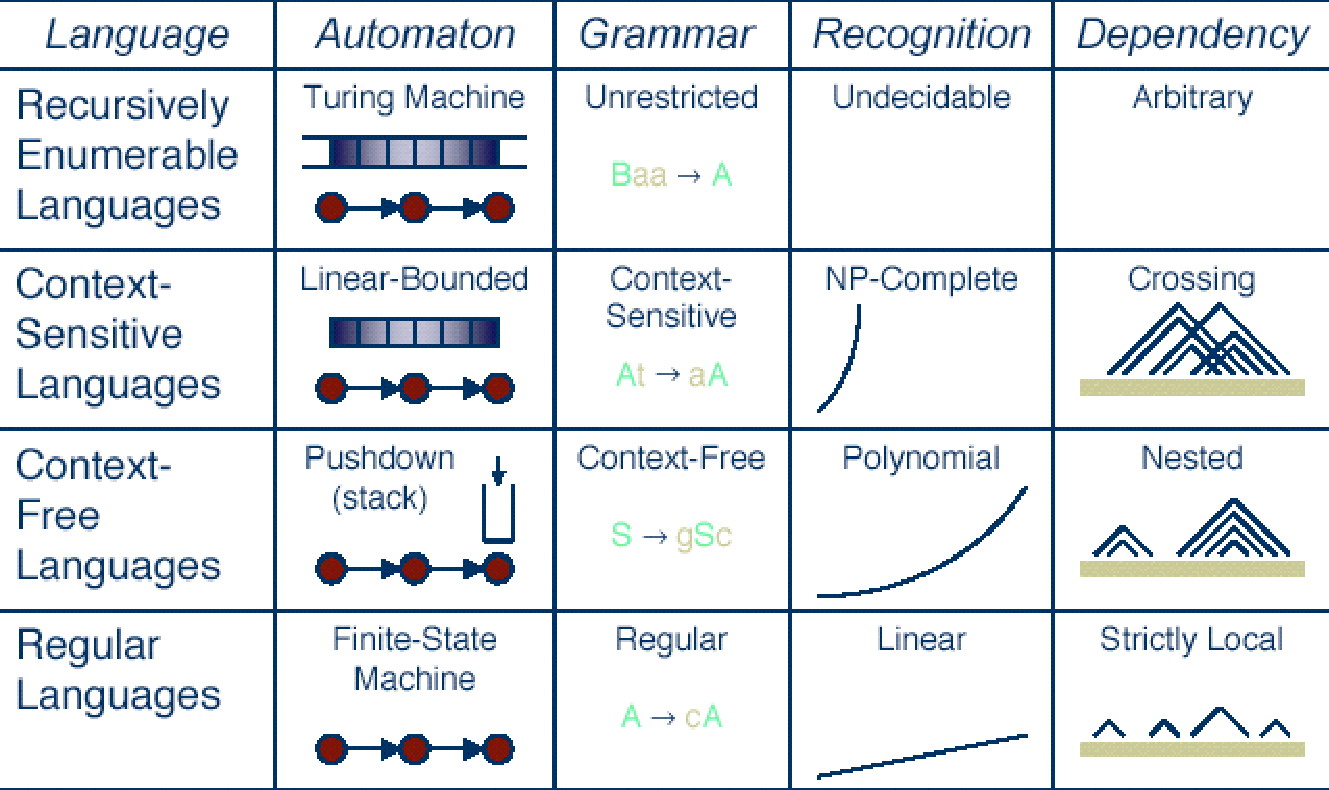
\includegraphics[width=8in]{chomskyhier}

\centering
TAG is between CSL and CFG: \\
has Polynomial time recognition and handles many crossing dependencies.

\end{center}
\end{slide}

\begin{slide}{\dbend\ Given grammar $G$ and input $x$, provide algorithm for: Is $x \in L(G)$?}
{\small \begin{itemize}
\item {\bf unrestricted}: {\color{red} undecidable} (grammars using `movement', feature structure unification)
\item {\bf context-sensitive}: {\color{red} NSPACE[n] -- linear non-deterministic space}
\item {\bf indexed} grammars: {\color{red} NP-Complete} (restricted feature structure unification)
\item {\bf tree-adjoining} grammars (TAG), {\bf linear-indexed}
  grammars (LIG), {\bf combinatory categorial} grammars (CCG), {\bf
  head} grammars: {\color{red} ${\cal O}(n^6)$} 
\item {\bf context-free}: {\color{red} ${\cal O}(n^3)$}
\item {\bf deterministic context-free}: {\color{red} ${\cal O}(n)$}
\item {\bf regular} grammars: {\color{red} ${\cal O}(n)$}
\end{itemize}}
Which class corresponds to human language?
\end{slide}

\begin{slide}{\dbend\ \underline{Tree Adjoining Grammars}}
\begin{itemize}
\item Membership is in P (${\cal O}(n^6)$)
\item TALs are closed under union, concatenation, Kleene closure, $h$,
  $h^{-1}$, intersection with RLs and regular substitution. There is
  also a pumping lemma for TALs (proofs in (VijayShanker, 1987))  \\
Tree Adjoining Languages are a full abstract family of languages
  (AFL) 
\item No equivalent of Ogden's Lemma. TALs are not closed under
  intersection, intersection with CFLs and complementation.
\item TAGs, LIGs, CCGs, HGs (see previous slide) were shown by TAG
  researchers to be {\bf weakly equivalent} (VijayShanker, 1987; Weir, 1988)
\end{itemize}
\end{slide}

\begin{slide}{\underline{Computationally Constrained Grammar Formalisms}}
\begin{itemize}
\item Why bother with computationally constrained grammar formalisms?
\item Perhaps linguists can analyze language free of any thoughts about computational efficiency, using any system that can elegantly explain the data
\item And then if at all necessary this analysis can be translated to a computationally constrained formalism
\end{itemize}
\end{slide}

\begin{slide}{\underline{Computationally Constrained Grammar Formalisms}}
\begin{itemize}
\item But what if the computational system actually provides constraints on what can and cannot happen?
\item The linguist would be forced to assume ad-hoc restrictions to adequately explain the facts
\item Better to start with a constrained system and grow only if necessary (Occam's Razor)
\item Read: (Gazdar, 1981, Linguistic Inquiry) and Remarks and Replies by E. Willams
\end{itemize}
\end{slide}

\begin{slide}{\underline{Overview}}
\begin{itemize}
\item Tree Adjoining Grammars \[ \textrm{TAGs} \left\{ 
\begin{array}{l}
\textrm{\strike{Weak vs. Strong Generative Capacity}}\\
\textrm{\strike{Natural Language and Complexity}}\\
\textrm{Lexicalization of Grammars}
\end{array}
\right. \]
\item TAGs for Natural Languages
%%\item TAGs for Biological Sequences
\end{itemize}
\end{slide}

\begin{slide}{\underline{Lexicalization of Grammars}}
\begin{itemize}
\item Why is lexicalization important? Here's a strange fact: a context-free grammar can be {\em infinitely} ambiguous.
\item Lexicalization of a grammar means that each elementary object is associated with some terminal symbol. This guarantees that every input is only {\em finitely ambiguous}.\\
(Joshi and Schabes, 1997) show TALs are {\em closed} under lexicalization: every TAL has a lexicalized grammar without changing the language.
\item Lexicalization is an interesting idea for syntax, semantics (in linguistics) and sentence processing (in psycholinguistics):\\
{\em What if each word brings with it an entire syntactic and semantic context for that word?}
\end{itemize}
\end{slide}

\begin{slide}{\underline{Lexicalization of Context-Free Grammars}}
\begin{itemize}
\item Can we transform every CFG to a normal form where there is
  guaranteed to be a terminal symbol on the right hand side?
\item Answer: {\color{blue} yes} -- using Griebach Normal Form
\item Every CFG can be converted to the form: $A \rightarrow a\
  \alpha$ where $A$ is a non-terminal, $a$ is a terminal symbol, and
  $\alpha \in N^\ast$
\end{itemize}
\end{slide}

\begin{slide}{\underline{Griebach Normal Form: $T(G) \neq T(GNF(G))$}}
\begin{eqnarray}
A_1 & \rightarrow & A_2\ A_3 \nonumber \\
A_2 & \rightarrow & A_3\ A_1 \mid b \nonumber \\
A_3 & \rightarrow & A_1\ A_2 \mid a\nonumber 
\end{eqnarray}
\begin{center}
\includegraphics[height=3in]{figures.33}
\end{center}
\end{slide}

\begin{slide}{\underline{Lexicalization of Context-Free Grammars}}
\begin{itemize}
\item CFG $G$: ($r_1$) $S \rightarrow\ S\ S$\ \ \ \ ($r_2$) $S \rightarrow\ a$
\item Tree substitution Grammar $G'$:\\\ 
\\
\includegraphics[height=2.8in]{figures.9}
\end{itemize}
\end{slide}

\begin{slide}{\underline{Lexicalization of Context-Free Grammars}}
\begin{center}
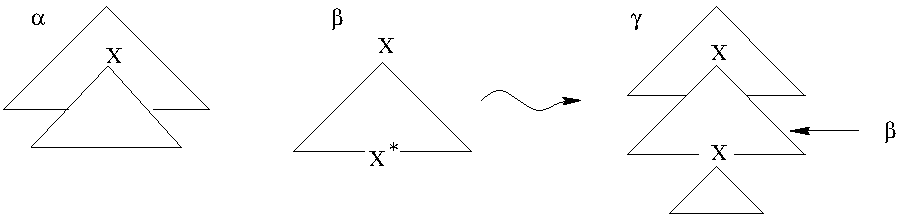
\includegraphics[height=2.25in]{adjunction}
\end{center}
\end{slide}

\begin{slide}{\underline{Lexicalization of Context-Free Grammars}}
\begin{itemize}
\item CFG $G$: ($r_1$) $S \rightarrow\ S\ S$\ \ \ \ ($r_2$) $S \rightarrow\ a$
\item {\bf Lexicalized} Tree adjoining Grammar $G''$:\\\ 
\\
\includegraphics[height=2.8in]{figures.10}
\end{itemize}
\end{slide}

\begin{slide}{\underline{Overview}}
\begin{itemize}
\item Tree Adjoining Grammars \[ \textrm{TAGs} \left\{ 
\begin{array}{l}
\textrm{\strike{Weak vs. Strong Generative Capacity}}\\
\textrm{\strike{Natural Language and Complexity}}\\
\textrm{\strike{Lexicalization of Grammars}}
\end{array}
\right. \]
\item TAGs for Natural Languages
%%\item TAGs for Biological Sequences
\end{itemize}
\end{slide}

\begin{slide}{\underline{Lexicalized Tree Adjoining Grammars}}
\begin{itemize}
\item Finite set of elementary trees, such that each tree has at least
  one terminal symbol
\item Elementary trees: initial and auxiliary
\item Operations: substitution and adjunction
\item Derivation Tree: how elementary trees are put together
\item Derived Tree
\end{itemize}
\end{slide}

\begin{slide}{\underline{Localization of Dependencies}}
\begin{itemize}
\item Syntactic: 
\begin{itemize}
\item agreement: person, number, gender
\item subcategorization: sleeps (null), eats (NP); gives (NP NP)
\item filler-gap: {\color{blue} who} did John ask Bill to invite
  {\color{blue} $\epsilon$}
\item word order: within and across clauses as in scrambling, clitic
  movement, etc. 
\end{itemize}
\end{itemize}
\end{slide}

\begin{slide}{\underline{Localization of Dependencies}}
\begin{itemize}
\item Semantic: 
\begin{itemize}
\item function-argument: all arguments of the anchoring word (the {\em
  functor}) are localized
\item word clusters (flexible idioms): non-compositional,
  e.g. {\color{blue} take a walk, give a cold shoulder to}
\item word co-occurences, lexical semantic aspects of meaning
\end{itemize}
\end{itemize}
\end{slide}

\begin{slide}{\underline{Lexicalized Tree Adjoining Grammars}}
\begin{center}
\includegraphics[height=4in]{figures.11}
\end{center}
\end{slide}

\end{document}
